\documentclass[12pt]{fphw}
%\usepackage{mathpazo}
%\usepackage[utf8]{inputenc}
%\usepackage[T1]{fontenc}
\usepackage{sectsty}
\usepackage{graphicx}
\usepackage{booktabs}
\usepackage{listings}
\usepackage{enumerate}
\usepackage{xcolor}

\sectionfont{\bfseries\large\raggedright}

\definecolor{codegreen}{rgb}{0,0.6,0}
\definecolor{codegray}{rgb}{0.5,0.5,0.5}
\definecolor{codepurple}{rgb}{0.58,0,0.82}
\definecolor{backcolour}{rgb}{0.95,0.95,0.92}

\title{Experiment 1}
\author{Aditya Kumar (24MAI14003)\\}
\date{02 Aug, 2024}
\institute{Chandigarh University\\Master of Engineeing---Artificial Intelligence}
\class{Advanced Data Structures and Algorithms Lab (24CSH-622)\\}
\professor{Dr. Manjit Singh}

\begin{document}

\maketitle

\section*{}
\begin{problem}
  \textbf{Aim: }Write a program for the implementation of the following searching techniques on Linear Data Structures
  \begin{enumerate}
    \item Linear Search
    \item Binary Search
  \end{enumerate}
\end{problem}

\section{Theory}
\subsection{Linear Search}
Linear search is a simple search algorithm that checks every element in a list or array sequentially until the target element is found or the end of the list is reached. It has a time complexity of O(n) in the worst case, where n is the number of elements in the list. Linear search is useful when dealing with unsorted lists or arrays. 

\subsection{Binary Search}
Binary search is a more efficient search algorithm that works on sorted lists or arrays. It repeatedly divides the search interval in half until the target element is found or the search interval is empty. The time complexity of binary search is O(log n) in the worst case. Binary search is useful when dealing with sorted lists or arrays.

\section{Algorithm}
\subsection{Linear Search}
\begin{enumerate}
  \item Start at the beginning of the list.
  \item Compare the target element with the current element.
  \item If the target element is found, return the index of the element.
  \item If the target element is not found, move to the next element.
  \item Repeat steps 2-4 until the end of the list is reached.
  \item If the target element is not found, return -1.
\end{enumerate}
\subsection{Binary Search}
\begin{enumerate}
  \item Initialize the left and right pointers to the start and end of the list, respectively.
  \item Calculate the middle index as the average of the left and right pointers (rounded down).
  \item Compare the target element with the middle element.
  \item If the target element is found, return the middle index.
  \item If the target element is smaller than the middle element, update the right pointer to the middle index - 1.
  \item If the target element is larger than the middle element, update the left pointer to the middle index + 1.
  \item Repeat steps 2-6 until the target element is found or the left pointer is greater than the right pointer.
  \item If the target element is not found, return -1.
\end{enumerate}
\section{Code}
    \lstinputlisting[language=c++, backgroundcolor=\color{backcolour}, numbers=left, tabsize=2,basicstyle=\ttfamily\footnotesize]{e1.cc}
\section{Output}
  \begin{center}
    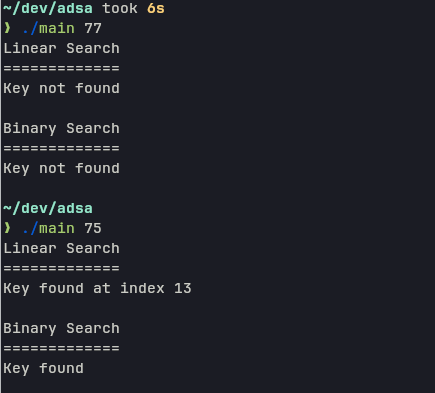
\includegraphics[width=0.5\columnwidth]{./e1.png}
  \end{center}
\section{Learning Outcomes}
\begin{enumerate}
  \item Understand the concepts and differences between linear search and binary search.
  \item Implement both algorithms in their preferred programming language.
  \item Apply linear search and binary search to solve problems involving searching for elements in lists or arrays.
  \item Recognize the importance of using binary search for sorted lists or arrays due to its more efficient time complexity compared to linear search.
\end{enumerate}
\end{document}
